\documentclass[a4paper,11pt,landscape,twocolumn]{article}

\usepackage{préambule}
\usepackage{clipboard}
\usetikzlibrary{calc}

\DeclareFontFamily{U}{skulls}{}
\DeclareFontShape{U}{skulls}{m}{n}{ <-> skull }{}
\newcommand{\skull}{\text{\usefont{U}{skulls}{m}{n}\symbol{'101}}}

\newcommand{\myAdd}[2]{\directlua{tex.print(#1 + #2)}}

\begin{luacode}
	function print_items(points)
		for _, p in ipairs(points) do
			tex.sprint("\\item (", p.x, "; ", p.y, ")")
		end
	end

	function print_path(points)
		tex.sprint("\\draw[red,thick] ")
		for i, p in ipairs(points) do
		 	if i ~= 1 then
		 		tex.sprint(" -- ")
		 	end
		 	tex.sprint("(", p.x, ",", p.y, ")")
		end
		tex.sprint(";")
	end
\end{luacode}

\begin{document}

\Copy{beta}{
	\directlua{
		points = {
				{ x = -7, y = 6 },
				{ x = -2, y = 1 },
				{ x = -2, y = -2 },
				{ x = -6, y = -2 },
				{ x = -6, y = -4 },
				{ x = 0, y = -4 },
				{ x = 0, y = 0 },
				{ x = 3, y = 0 },
				{ x = 6, y = 3 },
				{ x = 6, y = 6 },
				{ x = 7, y = 6 },
			}
	}

	{\large \textbf{Coordonnées γ :}}
	Ton camarade a la même carte, mais il ne sait pas qu'il y a des monstres sur certaines voies ! \\
	Décris-lui un chemin qui évite les monstres ({\color{red} \circled{\skull}}).

	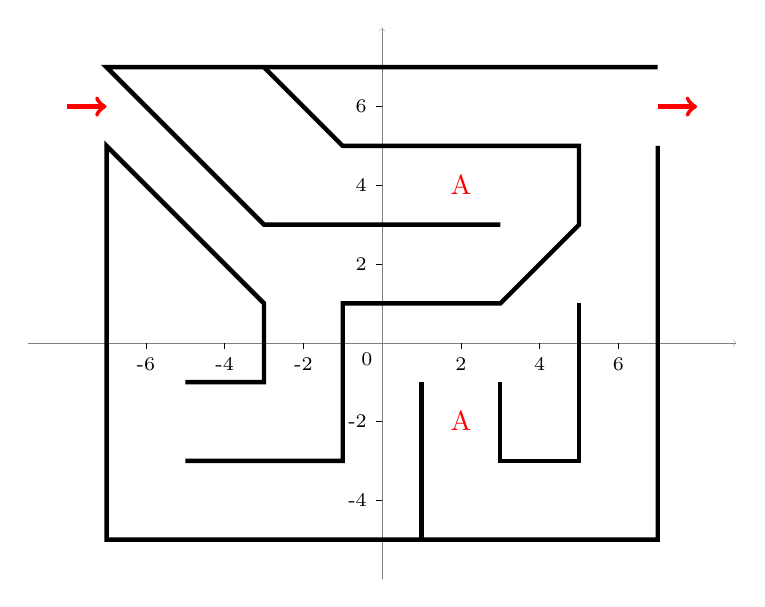
\begin{tikzpicture}[scale=0.5]
		\draw[gray,ultra thin,->] (-9,0) -- (9,0);
		\draw[gray,ultra thin,->] (0,-6) -- (0,8);
		\node[below left] at (0,0) {\scriptsize 0};

		\foreach \x in {-6,-4,-2,2,4,6} {
				\draw[very thin] (\x,0) -- (\x,-0.15) node[below] {\scriptsize \x};
			}

		\foreach \y in {-4,-2,2,4,6} {
				\draw[very thin] (0,\y) -- (-0.15,\y) node[left] {\scriptsize \y};
			}

		\draw[ultra thick,red,->] (-8,6) -- (-7,6);
		\draw[ultra thick,red,->] (7,6) -- (8,6);

		\draw[ultra thick] (-5,-1) -- (-3,-1) -- (-3,1) -- (-7, 5) -- (-7,-5) -- (7,-5) -- (7,5);
		\draw[ultra thick] (-5,-3) -- (-1,-3) -- (-1,1) -- (3,1) -- (5,3) -- (5,5) -- (-1,5) -- (-3,7);
		\draw[ultra thick] (1,-1) -- (1,-5);
		\draw[ultra thick] (3,-1) -- (3,-3) -- (5,-3) -- (5,1);
		\draw[ultra thick] (3,3) -- (-3,3) -- (-7,7) -- (7,7);

		\node[red] at (2,4) {\circled{\skull}};
		\node[red] at (2,-2) {\circled{\skull}};
	\end{tikzpicture}

	\hrule
	\vspace{1em}

	\textbf{Labyrinthe γ :} \vspace{1em}

	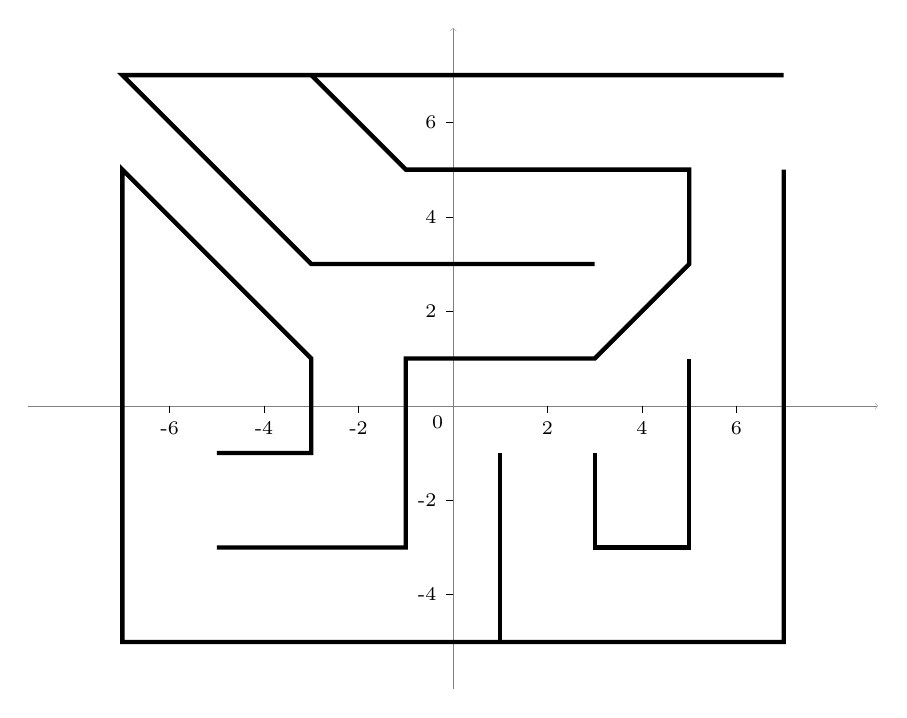
\begin{tikzpicture}[scale=0.6]
		\draw[gray,ultra thin,->] (-9,0) -- (9,0);
		\draw[gray,ultra thin,->] (0,-6) -- (0,8);
		\node[below left] at (0,0) {\scriptsize 0};

		\foreach \x in {-6,-4,-2,2,4,6} {
				\draw[very thin] (\x,0) -- (\x,-0.15) node[below] {\scriptsize \x};
			}

		\foreach \y in {-4,-2,2,4,6} {
				\draw[very thin] (0,\y) -- (-0.15,\y) node[left] {\scriptsize \y};
			}

		\draw[ultra thick] (-5,-1) -- (-3,-1) -- (-3,1) -- (-7, 5) -- (-7,-5) -- (7,-5) -- (7,5);
		\draw[ultra thick] (-5,-3) -- (-1,-3) -- (-1,1) -- (3,1) -- (5,3) -- (5,5) -- (-1,5) -- (-3,7);
		\draw[ultra thick] (1,-1) -- (1,-5);
		\draw[ultra thick] (3,-1) -- (3,-3) -- (5,-3) -- (5,1);
		\draw[ultra thick] (3,3) -- (-3,3) -- (-7,7) -- (7,7);

		% \directlua{print_path(points)}
	\end{tikzpicture}
}

\newpage

\Paste{beta}

\end{document}